\documentclass[oneside,reqno]{amsart}

\usepackage[utf8]{inputenc}
\usepackage{amsthm,mathtools,stmaryrd,amssymb,graphicx,ragged2e}
\usepackage{tikz}
\usetikzlibrary{calc,shapes,shapes.callouts,shapes.arrows,patterns,fit,backgrounds,decorations.pathmorphing}
\usepackage{booktabs,framed}
\usepackage[all]{xy}
\usepackage[protrusion=true,expansion=true]{microtype}
\usepackage{xspace}

\usepackage[natbib=true,style=numeric,maxnames=10]{biblatex}
\usepackage[babel]{csquotes}
\bibliography{paper-filmat.bib}

\graphicspath{{images/}}

\usepackage{pifont}
\newcommand{\cmark}{\ding{51}}
\newcommand{\xmark}{\ding{55}}
\definecolor{mypurple}{RGB}{150,0,255}

\title[]{Exploring mathematical objects from custom-tailored mathematical universes}
\author{Ingo Blechschmidt}
\address{Universität Augsburg \\
Institut für Mathematik \\
Universitätsstr. 14 \\
86159 Augsburg, Germany}
\email{ingo.blechschmidt@math.uni-augsburg.de}

\theoremstyle{definition}
\newtheorem{defn}{Definition}[section]
\newtheorem{ex}[defn]{Example}

\theoremstyle{plain}
\newtheorem{prop}[defn]{Proposition}
\newtheorem{cor}[defn]{Corollary}
\newtheorem{lemma}[defn]{Lemma}
\newtheorem{thm}[defn]{Theorem}
\newtheorem{scholium}[defn]{Scholium}

\theoremstyle{remark}
\newtheorem{rem}[defn]{Remark}
\newtheorem{question}[defn]{Question}
\newtheorem{speculation}[defn]{Speculation}
\newtheorem{caveat}[defn]{Caveat}
\newtheorem{conjecture}[defn]{Conjecture}

\newenvironment{indentblock}{%
  \list{}{\leftmargin\leftmargin}%
  \item\relax
}{%
  \endlist
}

\newcommand{\E}{\mathcal{E}}
\newcommand{\B}{\mathcal{B}}
\newcommand{\BB}{\mathbb{B}}
\newcommand{\NN}{\mathbb{N}}
\newcommand{\QQ}{\mathbb{Q}}
\newcommand{\TT}{\mathbb{T}}
\newcommand{\RR}{\mathbb{R}}
\newcommand{\ZZ}{\mathbb{Z}}
\renewcommand{\P}{\mathcal{P}}
\renewcommand{\O}{\mathcal{O}}
\newcommand{\defeq}{\vcentcolon=}
\newcommand{\op}{\mathrm{op}}
\DeclareMathOperator{\Spec}{Spec}
\DeclareMathOperator{\Hom}{Hom}
\DeclareMathOperator{\Mod}{Mod}
\DeclareMathOperator{\Sh}{Sh}
\DeclareMathOperator{\Zar}{Zar}
\DeclareMathOperator{\PSh}{PSh}
\newcommand{\Set}{\mathrm{Set}}
\newcommand{\Eff}{\mathrm{Ef{}f}}
\renewcommand{\_}{\mathpunct{.}\,}
\newcommand{\effective}{ef{}fective\xspace}
\newcommand{\effectively}{ef{}fectively\xspace}
\newcommand{\?}{\,{:}\,}
\newcommand{\realizes}{\Vdash}
\newcommand{\notnot}{\emph{not~not}\xspace}
\newcommand{\seq}[1]{\mathrel{\vdash\!\!\!_{#1}}}

\newcommand{\stacksproject}[1]{\cite[{\href{https://stacks.math.columbia.edu/tag/#1}{Tag~#1}}]{stacks-project}}

\renewcommand{\paragraph}[1]{\noindent\textbf{#1.}}

\begin{document}

\begin{abstract}
  XXX
\end{abstract}

\maketitle
\thispagestyle{empty}

\tableofcontents

\noindent
Toposes can be pictured as mathematical universes in which we can do
mathematics. Most mathematicians spend all their professional life in just a
single topos, the so-called \emph{standard topos}. However, besides the
standard topos, there is a colorful host of alternate toposes which are just as
worthy of mathematical study and in which mathematics plays out slightly
differently (Figure~\ref{fig:landscape}).

\begin{figure}
  \tikzstyle{topos} = [draw=mypurple, very thick, rectangle, rounded corners, inner sep=5pt, inner ysep=10pt]
  \tikzstyle{title} = [fill=mypurple, text=white]

  % Taken from Todd Lehman (CC-BY-SA) at https://tex.stackexchange.com/a/44920/32372

\newcommand{\setisprime}[1]{
  % Sets \isprime based on #1.
  \ifnum#1=1 \gdef\isprime{0} \else \gdef\isprime{1} \fi
  \foreach \sip in {2, 3,5,...,#1} {
    \pgfmathparse{\sip*\sip>#1? 1:0}
    \ifthenelse{\pgfmathresult=1}{
      % Early-out if \sip^2 > #1.
      \breakforeach
    }{
      % Otherwise test if \sip divides #1.
      \pgfmathparse{Mod(#1,\sip)==0? 1:0}
      \ifthenelse{\pgfmathresult=1}{
        \gdef\isprime{0}
        \breakforeach
      }{}
    }
  }
}

\newcommand{\setxy}[1]{
  % Sets \x and \y to loction of cell #1.
  \pgfmathtruncatemacro{\x}{Mod(#1-1,\cols)}
  \pgfmathtruncatemacro{\y}{(#1-1) / \cols}
  \pgfmathtruncatemacro{\y}{\cols - 1 - \y}
  \pgfmathparse{2.5*(\x+.5)}\let\x\pgfmathresult
  \pgfmathparse{2.5*(\y+.5)}\let\y\pgfmathresult
}

\newcommand{\numlabel}[2]{
  % Draws label #2 at cell #1.
  \setxy{\n}
  \node[fill=none, text=black] at (\x,\y) {#2};
}

\newcommand{\drawpolygon}[2]{
  % Draws polygon with #2 vertexes at cell #1.
  \setxy{#1}
  \ifthenelse{#2>1}{ % Polygon must have at least 2 sides.
    \ifthenelse{#2<30}{ % Draw polygon if it has a small number of sides.
      \filldraw (\x,\y) +(90:1)
      \foreach \drawi in {1,...,#2} {-- +(\drawi/#2*360+90:1)} -- cycle;
    }{ % Else approximate with circle.
      \filldraw (\x,\y) circle(1);
    }
  }{}
}

\newcommand{\setpolygoncolor}[1]{
  % Sets color based on #1.
  \gdef\polycolor{black}
  \ifnum#1=2\gdef\polycolor{black!50!white}\fi
  \ifnum#1=3\gdef\polycolor{yellow!95!red}\fi
  \ifnum#1=5\gdef\polycolor{yellow!0!red}\fi
  \ifnum#1=7\gdef\polycolor{blue!75!green}\fi
  \ifnum#1=11\gdef\polycolor{blue!70!red}\fi
  \ifnum#1=13\gdef\polycolor{blue!40!red}\fi
  \ifnum#1=17\gdef\polycolor{green!50!blue}\fi
  \ifnum#1=19\gdef\polycolor{green!80!black}\fi
  \ifnum#1=23\gdef\polycolor{green!50!red}\fi
  \ifnum#1=29\gdef\polycolor{yellow!50!black}\fi
  \ifnum#1=31\gdef\polycolor{orange!50!black}\fi
  \ifnum#1=37\gdef\polycolor{red!50!black}\fi
  \ifnum#1=41\gdef\polycolor{purple!50!black}\fi
  \ifnum#1=43\gdef\polycolor{blue!50!black}\fi
  \ifnum#1=47\gdef\polycolor{green!50!black}\fi
  \ifnum#1=53\gdef\polycolor{white!50!black}\fi
  \ifnum#1=59\gdef\polycolor{white!50!black}\fi
  \ifnum#1=61\gdef\polycolor{white!50!black}\fi
  \ifnum#1=67\gdef\polycolor{white!50!black}\fi
}

\newcommand{\sieve}[2]{
  \def\cols{#1}
  \def\rows{#2}
  \begin{tikzpicture}[scale=.5]
  \pgfmathtruncatemacro{\nmax}{\rows * \cols}

  \foreach \n in {1,...,\nmax} {
    \begin{scope}[fill=gray, fill opacity=.05,
                  draw=gray, draw opacity=.10,
                  line width=4]
      \drawpolygon{\n}{\n}
    \end{scope}
    \setisprime{\n}
    \ifthenelse{\isprime=1}{
      \numlabel{\n}{\bf\n}
    }{
      \def\startintensity{.33}
      \def\incrintensity{.10}
      \def\intensity{\startintensity}

      \def\m{\n}
      \pgfmathtruncatemacro{\i}{\m / 2}

      % Divide \m by \i until \m is extinguished.
      % Increment \i each time it does not divide into \m.
      \whiledo{\m>1}{
        \setisprime{\i}
        \pgfmathparse{Mod(\m,\i)==0? 1:0}
        \ifthenelse{\pgfmathresult=1\and\isprime=1}{
          \setpolygoncolor{\i}
          \begin{scope}[fill=\polycolor, fill opacity=\intensity,
                        draw=\polycolor!85!black, draw opacity=\intensity,
                        line width=\intensity*1.5]
            \drawpolygon{\n}{\i}
          \end{scope}
          \pgfmathtruncatemacro{\m}{\m / \i}
          \pgfmathparse{\intensity + \incrintensity}\let\intensity\pgfmathresult
        }{
          \pgfmathtruncatemacro{\i}{\i - 1}
          \def\intensity{\startintensity}
        }
      }
      \begin{scope}[text=black, text opacity=.5]
        \numlabel{\n}{\scriptsize\n}
      \end{scope}
    }
  }

  \end{tikzpicture}
}


  \newcommand{\drawbox}[4]{
    \node[topos, #4] [fit = #3] (#1) {};
    \node[title] at (#1.north) {#2};
  }

  \newcommand{\muchstuff}{
    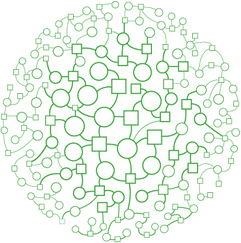
\includegraphics[height=3em]{filmat}
    \scalebox{0.5}{\sieve{14}{2}}
  }

  \newcommand{\muchstuffplaceholder}{
    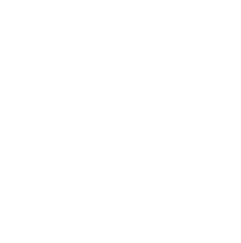
\includegraphics[height=3em]{filmat-placeholder}
    \scalebox{0.5}{\fakesieve{14}{2}}
  }

  \newcommand{\fewstuff}{
    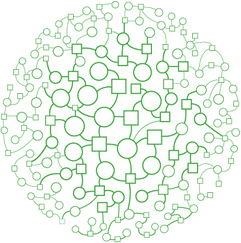
\includegraphics[height=3em]{filmat}
    \scalebox{0.5}{\sieve{7}{2}}
  }

  \newcommand{\threeblobs}{
    \colorbox{mypurple}{\ \ }\quad
    \colorbox{mypurple}{\ \ }\quad
    \colorbox{mypurple}{\ \ }
  }

  \begin{tikzpicture}
    \node (objs-set0) at (0,0) {
      \muchstuff
    };
    \node[scale=0.4] (objs-set1) at (-3.5,-2.5) {
      \fewstuff
    };
    \node[scale=0.4] (objs-eff1) at (3.5,-2.5) {
      \fewstuff
    };
    \node[scale=0.4] (objs-sh1)  at (0,-2.5) {
      \fewstuff
    };

    \node (prop-set1) [below of=objs-set1, align=left] {
      The usual laws \\
      of logic hold.
    };

    \node (prop-eff1) [below of=objs-eff1, align=left] {
      Every function \\
      is computable.
    };

    \node (prop-sh1) [below of=objs-sh1, align=left] {
      The axiom of \\
      choice fails.
    };

    \node (more-eff1) [below of=prop-eff1] {
      \threeblobs
    };
    \node (more-sh1)  [below of=prop-sh1] {
      \threeblobs
    };
    \node (more-set1) [below of=prop-set1] {
      \threeblobs
    };

    \drawbox{set1}{$\mathrm{Set}$}{(objs-set1) (prop-set1) (more-set1)}{}
    \drawbox{eff1}{Ef{}f}{(objs-eff1) (prop-eff1) (more-eff1)}{tape}
    \drawbox{sh1}{$\mathrm{Sh}\, X$}{(objs-sh1) (prop-sh1) (more-sh1)}{draw=none}
    \def\R{8pt}
    \begin{pgfonlayer}{background}
    \draw[decoration={bumps,segment length=8pt}, decorate, very thick, draw=mypurple]
      ($(sh1.south west) + (\R, 0)$) arc(270:180:\R) --
      ($(sh1.north west) + (0, -\R)$) arc(180:90:\R) --
      ($(sh1.north east) + (-\R, 0)$) arc(90:0:\R) --
      ($(sh1.south east) + (0, \R)$) arc(0:-90:\R) --
      cycle;
    \end{pgfonlayer}
    \drawbox{set0}{$\mathrm{Set}$}{(objs-set0) (set1) (eff1) (sh1)}{}
  \end{tikzpicture}

  \caption{\label{fig:landscape}A glimpse of the toposophic landscape,
  displaying alongside the standard topos~$\Set$ two further toposes.}
  % Each topos comes with its own copy of the natural numbers and all the other
  % familiar mathematical objects.
  % Toposes are still mathematical structures and hence part of the standard
  % topos, which is why the standard topos is also drawn to encompass ...
\end{figure}

% \begin{document}

For instance, there are toposes in which the axiom of choice and the
intermediate value theorem from undergraduate calculus fail, toposes in which
any function~$\RR \to \RR$ is continuous and toposes in which infinitesimal
numbers exist.

The purpose of this contribution is twofold.
\begin{enumerate}
\item We give a glimpse of the toposophic landscape, presenting several
specific toposes and exploring their peculiar properties.

\item We explicate how toposes provide distinct lenses through which the
usual mathematical objects of the standard topos can be viewed.
\end{enumerate}
% XXX check everywhere

Viewed through such a lens, a given mathematical object can have different
properties than when considered normally. In particular, it can have
better properties for the purposes of specific applications, especially if
the topos is custom-tailored to the object in question. This change of
perspective has been used in mathematical practice and demonstrates that
toposes go much beyond being logicians' testbeds. To give just a taste of what
is possible, through the lens provided by an appropriate topos, any given ring
can look like a field and hence mathematical techniques for fields also apply,
through the lens, to rings.

We argue that toposes and specifically the change in perspective provided by
toposes are ripe for philosophical analysis. In particular, there are the
following connections with topics in the philosophy of mathematics:
\begin{enumerate}
\item Toposes enrich the realism/anti-realism debate in that they paint the larger
picture that the platonic heaven of mathematical objects is not unique: besides
the standard heaven of the standard topos, we can fathom the alternate
heavens of all other toposes, all embedded in a second-order heaven.
\item Mathematics is not only about studying mathematical objects, but also
about studying the relations between mathematical objects. The distinct view
on mathematical objects provided by any topos uncovers relations which
otherwise remain hidden.
% XXX: mention Olivia?
\item In some cases, a mathematical relation can be expressed quite succinctly
using the language of a specific topos and not so succinctly using the language
of the standard topos. This phenomenon showcases the importance of
\emph{appropriate language}.
\item Toposes provide new impetus to study constructive mathematics and
intuitionistic logic, in particular also to restrict to intuitionistic
logic on the meta level and to consider the idea that the platonic heaven might
be governed by intuitionistic logic.
% XXX contingent: To some extent, what the commonly agreed-upon rules of
% mathematics are is dependent on contingent historical factors. It is
% conceivable, for instance, that the intuitionists ...
\end{enumerate}
This note touches on these topics and invites further research.

\bigskip
\paragraph{Acknowledgments} We are grateful to XXX for many invaluable
discussions shaping this work and to XXX for their careful criticism of earlier
drafts. XXX conference organizer and participants
% Todd Lehman for creating parts of Figure~1


\section{Toposes as alternate mathematical universes}

Formally, a topos is a certain kind of \emph{category}, containing objects and
morphisms between those objects. The formal definition, recorded here only for
reference, requires some amount of category theory, but, as will be outlined in
the following sections, exploring the mathematical universe of a given topos
does not.

\begin{defn}A \emph{topos} (more precisely \emph{elementary topos} or
\emph{logos} with a natural numbers object) is a category which has all finite
limits, is cartesian closed, has a subobject classifier and contains a natural
numbers object.\end{defn}

Put briefly, these axioms state that a topos should share several categorical
properties with the category of sets; they ensure that each topos contains its
own versions of familiar mathematical objects such as natural numbers, real
numbers, groups and manifolds, and is closed under the usual constructions
such as cartesian products or quotients.
The prototypical topos is the standard topos:

\begin{defn}The \emph{standard topos}~$\Set$ is the category which contains all
sets as its objects and all maps between sets as morphisms.\end{defn}

Given a topos~$\E$, we write~``$\E \models \varphi$'' to denote that a
mathematical statement~$\varphi$ \emph{holds in~$\E$}. The meaning of~``$\E \models
\varphi$'' is defined by recursion on the structure of~$\varphi$ following the
so-called \emph{Kripke--Joyal translation rules}. For instance, the rule for
translating conjunction reads
\[ \E \models (\alpha \wedge \beta) \qquad\text{iff}\qquad
  \E \models \alpha \quad\text{and}\quad \E \models \beta. \]
The remaining translation rules are more involved; we do not list them here for
the case of a general topos~$\E$, but we will state them in the next sections
for several specific toposes.

In the definition of~$\E \models \varphi$, the statement~$\varphi$ can be any
statement in the language of a general version of higher-order predicate
calculus with dependent types. In practice almost any mathematical statement
can be interpreted in a given topos.\footnote{The main exceptions are
statements from set theory, which typically make substantial use of a global
membership predicate~``$\in$''. Toposes only support a typed \emph{local}
membership predicate, where we may write~``$x \in A$'' only in the context of
some fixed type~$M$ such that~$x$ is of type~$M$ and~$A$ is of
type~$P(M)$, the power type of~$M$. We refer
to~\cite{fourman:sheaf-models,streicher:forcizf,awodey-butz-simpson-streicher:bist}
for ways around this restriction.}

It is by the Kripke--Joyal translation rules that we can access the alternate
universe of a topos. In the special case of the standard topos~$\Set$, the
definition of~``$\Set \models \varphi$'' unfolds to~$\varphi$ for any
statement~$\varphi$. Hence a statement holds in the standard topos if and only
if it holds in the usual mathematical sense.


\subsection{The logic of toposes} By their definition as special kinds of
categories, toposes are merely algebraic structures not unlike groups or vector
spaces. Hence we need to argue why we picture toposes as mathematical universes
while we do not elevate other kinds of algebraic structures in the same way.
For us, this usage is justified by the following metatheorem:

\begin{thm}\label{thm:reasoning}Let~$\E$ be a topos and let~$\varphi$ be a
statement such that~$\E \models \varphi$. If~$\varphi$ intuitionistically
entails a further statement~$\psi$ (that is, if it is provable in
intuitionistic logic that~$\varphi$ entails~$\psi$), then~$\E \models
\psi$.\end{thm}

This metatheorem allows us to \emph{reason} in toposes. When first exploring a
new topos~$\E$, we need to employ the Kripke--Joyal translation rules each time
we want to check whether a statement holds in~$\E$. But as soon as we
have amassed a stock of statements known to be true in~$\E$, we can find more
by deducing their logical consequences.

For instance, in any topos where the statement ``any map~$\RR \to \RR$ is
continuous'' is true, also the statement ``any map~$\RR \to \RR^2$ is
continuous'' is, since there is an intuitionistic proof that a map into a
higher-dimensional Euclidean space is continuous if its individual components
are.

The only caveat of Theorem~\ref{thm:reasoning} is that toposes generally only
support intuitionistic reasoning, not the full power of the ordinary
\emph{classical reasoning}. That is, within most toposes, the law of excluded
middle ($\varphi \vee \neg\varphi$) and the law of double negation elimination
($\neg\neg\varphi \Rightarrow \varphi$) are not available.

While it may appear that these two laws pervade any mathematical theory, in
fact a substantial amount of mathematics can be developed intuitionistically
(see for
instance~\cite{mines-richman-ruitenburg:constructive-algebra,lombardi-quitte:constructive-algebra}
for constructive algebra,~\cite{bishop-bridges:constructive-analysis} for
constructive analysis
and~\cite{bauer:int-mathematics,bauer:video,melikhov:intuitionistic-logic} for
further references) and hence the alternate universes provided by toposes
cannot be too strange: In any topos, there are infinitely many prime numbers,
the square root of two is not rational and the powerset of the naturals is
uncountable.

That said, intuitionistic logic still allows for a considerable amount of
freedom, and in many toposes statements are true which are baffling if one has
only received training in mathematics based on classical logic. For instance, on first sight it
looks like the signum function
\[ \operatorname{sgn} : \RR \longrightarrow \RR,\ x \longmapsto \begin{cases}
  -1, & \text{if $x < 0$,} \\
  0, & \text{if $x = 0$,} \\
  1, & \text{if $x > 0$,}
\end{cases} \]
is an obvious counterexample to the statement ``any map~$\RR \to \RR$ is
continuous''. However, closer inspection reveals that the signum function
cannot be proven to be a total function~$\RR \to \RR$ if only intuitionistic
logic is available. The domain of the signum
function is the subset~$\{ x \in \RR \,|\, x < 0 \vee x = 0 \vee x > 0 \}
\subseteq \RR$, and in intuitionistic logic this subset cannot be shown to
coincide with~$\RR$.

Sections~\ref{sect:effective-topos} to~\ref{sect:smooth} present several
examples for such anti-classical statements and explain how to make sense of
them. Some toposes are closer to the standard topos and do not validate such
anti-classical statements:

\begin{defn}A topos~$\E$ is \emph{boolean} if and only if the laws of classical
logic are true in~$\E$.\end{defn}

Since exactly those statements hold in the standard topos which hold on the
meta level, the standard topos is boolean if and only if, as is commonly supposed, the laws
of classical logic hold on the meta level. Most toposes of interest are not
boolean, irrespective of one's philosophical commitments about the meta level,
and conversely some toposes are boolean even if classical logic is not
available on the meta level.

\begin{rem}The axiom of choice (which is strictly speaking not part of
classical logic, but of classical set theory) is also not available in most
toposes. By \emph{Diaconescu's theorem}, the axiom of choice implies the law of
excluded middle in presence of other axioms which are available in any topos.
\end{rem}

%A natural question is this: \emph{Which of
%the familiar mathematical facts of the standard topos carry over to arbitrary
%toposes?} For any given mathematical statement~$\varphi$ and topos~$\E$,
%we can unroll the definition of~$\E \models \varphi$ to try to check
%whether~$\varphi$ holds in~$\E$ on an individual case-by-case basis; but since
%any topos supports intuitionistic reasoning, we may at once conclude: \emph{Any
%theorem of constructive mathematics, that is any theorem deduced using only
%intuitionistic logic, is valid in any topos.}

%Mathematicians are familiar with the fact that the usual objects of
%mathematical study are governed by the laws of ordinary \emph{classical
%reasoning}. ...


\subsection{Relation to models of set theory} In set theory, philosophy and
logic, models of set theories are studied. These are structures~$(M,\in)$
validating the axioms of some set theory such as Zermelo--Fraenkel set theory
with choice~\textsc{zfc}, and they can be pictured as ``universes in which we
can do mathematics'' in much the same way as toposes.

In fact, to any model~$(M,\in)$ of a set theory such as~\textsc{zf}
or~\textsc{zfc}, there is a topos~$\Set_M$ such that a statement holds
in~$\Set_M$ if and only if it holds in~$M$.\footnote{The topos~$\Set_M$ can be
described as follows: Its objects are the elements of~$M$, that is the entities
which~$M$ believes to be sets, and its morphisms are those entities which~$M$
believes to be maps. The topos~$\Set_M$ validates the axioms of the structural
set theory \textsc{etcs}~\cite{mclarty:structuralism,marquis:foundations,barton-friedman:structures}, and models are isomorphic if and only if their
associated toposes are equivalent as categories.}

\begin{ex}The topos~$\Set_V$ associated to the universe~$V$ of all sets (if
this structure is available in one's chosen ontology) coincides with the
standard topos~$\Set$.\end{ex}

In set theory, we use forcing and other techniques to construct new
models of set theory from given ones, thereby exploring the set-theoretic
multiverse. There are similar techniques available for constructing new toposes
from given ones, and some of these correspond to the techniques from set
theory.

However, there are also important differences between the notion of mathematical
universes as provided by toposes and as provided by models of set theory, both
regarding the subject matter and the reasons for why we are interested in them.

Firstly, toposes are more general than models of set theory. By definition, a
model of \textsc{zfc} will always satisfy the axioms of \textsc{zfc}; in
contrast, most toposes do not even validate the law of excluded middle, much
less so the axiom of choice.

Secondly, there is a shift in emphasis. An important philosophical objective
for studying models of set theory is to explore which notions of sets are
coherent: Does the cardinality of the reals need to be the cardinal directly
succeeding~$\aleph_0$, the cardinality of the naturals? No, there are models of
set theory in which the continuum hypothesis fails. Do non-measurable sets of
reals need to exist? No, in models of~$\textsc{zf}+\textsc{ad}$,
Zermelo--Fraenkel set theory plus the axiom of determinacy, it is a theorem that
every subset of~$\RR^n$ is Lebesgue-measurable. Can the axiom of choice be
added to the axioms of~\textsc{zf} without causing inconsistency? Yes, if~$M$
is a model of~\textsc{zf} then~$L^M$, the structure of the constructible sets of~$M$, forms a
model of~\textsc{zfc}.

Toposes can be used for similar such purposes, and indeed have been,
especially to explore the various intuitionistic notions of sets. However, an important
aspect of topos theory is that toposes are used to explore the \emph{standard}
mathematical universe: truth in the \effective topos tells us what is
computable; truth in sheaf toposes tells us what is true locally; toposes
adapted to synthetic differential geometry can be used to rigorously work with
infinitesimals. All of these examples will be presented in more detail in the
next sections.

In a sense which can be made precise, toposes allow us to study the usual
objects of mathematics from a different point of view -- one such view for
every topos -- and it is a beautiful and intriguing fact that with the sole
exception of the law of excluded middle, the laws of logic apply to
mathematical objects also when viewed through the lens of a specific topos.


\subsection{A glimpse of the toposophic landscape}
There is a proper class of toposes. Figure~\ref{fig:landscape} depicts three
toposes side by side: the standard topos, a sheaf topos and the \effective
topos. Each of these toposes tells a different story of mathematics, and any
topos which is not the standard topos invites us to ponder alternative ways how
mathematics could unfold.

Some of the most prominent toposes are the following.

\begin{enumerate}
\item The \emph{trivial topos}. In the trivial topos, any statement whatsoever
is true. The trivial topos is not interesting on its own, but its existence
streamlines the theory and it can be an interesting question whether a given
topos coincides with the trivial topos.
\item $\Set$, the \emph{standard topos}. A statement is true in~$\Set$ iff it is true
in the ordinary mathematical sense.
\item $\Set_M$, the topos associated to any model~$(M,\in)$ of~\textsc{zf}.
\item $\Eff$, the \emph{\effective topos}. A statement is true in~$\Eff$ iff
if it has a \emph{computable witness} as detailed in
Section~\ref{sect:effective-topos}. In~$\Eff$, any function~$\NN \to \NN$ is
computable, any function~$\RR \to \RR$ is continuous and the countable axiom of
choice holds (even if it does not on the meta level).
\item $\Sh(X)$, the \emph{topos of sheaves} over any space~$X$. A statement is true
in~$\Sh(X)$ iff it holds \emph{locally on~$X$}, as detailed in
Section~\ref{sect:sheaf-toposes}. For most choices of~$X$, the
axiom of choice and the intermediate value theorem fail in~$\Sh(X)$, and this
failure is for geometric reasons.
\item $\Zar(A)$, the \emph{Zariski topos} of a ring~$A$ presented in
Section~\ref{sect:smooth}. This topos contains a mirror
image of~$A$ which is a field, even if~$A$ is not.
\item $\mathrm{Bohr}(A)$, the \emph{Bohr topos} associated to a noncommutative
C\textsuperscript{*}\kern-.1ex-algebra~$A$. This topos contains a mirror image
of~$A$ which is commutative. In this sense, quantum mechanical systems (which are
described by noncommutative C\textsuperscript{*}\kern-.1ex-algebras) can be
regarded as classical mechanical systems (which are described by commutative
algebras)~\cite{butterfield-hamilton-isham:bohr,heunen-landsman-spitters:aqt}.
\item $\Set[\TT]$, the \emph{classifying topos} of a geometric theory~$\TT$.\footnote{A
geometric theory is a theory in many-sorted first-order logic whose axioms can be put as \emph{geometric
sequents}, sequents of the form~$\varphi \seq{\vec x} \psi$ where~$\varphi$
and~$\psi$ are geometric formulas (formulas built from equality and specified
relation symbols by the logical
connectives~${\top}\,{\bot}\,{\wedge}\,{\vee}\,{\exists}$ and by arbitrary
set-indexed disjunctions~$\bigvee$).} This topos contains the
\emph{generic~$\TT$-model}. For instance, the classifying topos of the theory
of groups contains the \emph{generic group}. Arguably it is this group
which we implicitly refer to when we utter the phrase ``Let~$G$ be a group.''.
The generic group has has exactly those
properties which are shared by any group whatsoever.\footnote{More precisely,
this is only true for those properties which can be formulated as geometric
sequents. For arbitrary properties~$\varphi$, the statements~``the generic
group has property~$\varphi$'' and~``all groups have property~$\varphi$'' need
not be equivalent. This situation is explored
in~\cite{blechschmidt:nullstellensatz}.}
% FUTURE: Give Set[T] its own section.
\item $T(\mathcal{L}_0)$, the \emph{free topos}. A statement is true in the free topos iff it is
intuitionistically provable. Lambek and Scott proposed that the free topos can
reconcile moderate platonism (because this topos has a certain universal
property which can be used to single it out among the plenitude of toposes),
moderate formalism (because it is constructed in a purely syntactic way) and
moderate logicism (because, as a topos, it supports an intuitionistic type
theory)~\cite{lambek:incompatible,couture-lambek:reflections}.
\end{enumerate}

There are several constructions which produce a new toposes from a given
topos~$\E$. A non-exhaustive list is the following.
\begin{enumerate}
\item Given an object~$X$ of~$\E$, the \emph{slice topos}~$\E/X$
contains a \emph{generic element}~$x_0$ of~$X$. This generic element can be
pictured as the element we implicitly refer to when we utter the
phrase~``Let~$x$ be an element of~$X$.''. A statement~$\varphi(x_0)$
about~$x_0$ is true in~$\E/X$ if and only if in~$\E$ the statement~$\forall x
\? X\_ \varphi(x)$ is true.

For instance, the topos~$\Set/\QQ$ contains the generic rational number~$x_0$.
Neither the statement~``$x_0$ is zero'' nor the statement~``$x_0$ is not zero''
hold in~$\Set/\QQ$, as it is neither the case that any rational number
in~$\Set$ is zero nor that any rational number in~$\Set$ is not zero. Like any
rational number, the number~$x_0$ can be written as a fraction~$\frac{a}{b}$.
Just as~$x_0$ itself, the numbers~$a$ and~$b$ are quite indetermined.
\item Given a statement~$\varphi$ (which may contain objects of~$\E$ as
parameters but which must be formalizable as a geometric sequent), there is a
largest subtopos of~$\E$ in which~$\varphi$ holds. This construction is useful
if neither~$\varphi$ nor~$\neg\varphi$ hold in~$\E$ and we want to
force~$\varphi$ to be true. If~$\E \models \neg\varphi$, then the resulting
topos is the trivial topos.
% FUTURE: The topos~$\E[\mathbb{O}]$ contains a \emph{generic object}.
\item There is a ``smallest dense'' subtopos $\Sh_{\neg\neg}(\E)$. This topos
is always boolean, even if~$\E$ and the meta level are not. For a mathematician who employs
intuitionistic logic on their meta level, the nonconstructive results of their
classical colleagues do not appear to make sense in~$\Set$, but they hold
in~$\Sh_{\neg\neg}(\Set)$. If classical logic holds on the meta level,
then~$\Set$ and~$\Sh_{\neg\neg}(\Set)$ coincide.

The topos~$\Sh_{\neg\neg}(\E)$ is related to the \emph{double negation
translation}~$\varphi \mapsto \varphi^{\neg\neg}$ from classical logic into
intuitionistic logic: A statement~$\varphi$ holds in~$\Sh_{\neg\neg}(\E)$ if
and only if~$\varphi^{\neg\neg}$ holds
in~$\E$~\cite[Theorem~6.31]{blechschmidt:phd}.
% FUTURE: ultrapowers, gluing
\end{enumerate}

Toposes are still mathematical structures, and as long as we study
toposes within the usual setup of mathematics, our toposes are all part of the
standard topos. This is why Figure~\ref{fig:landscape} pictures the standard
topos twice. Hence the toposes which we can study in mathematics do not tell us
all possible stories how mathematics could unfold, only those which appear
coherent from the point of view of the standard topos, and the topos-theoretic
multiverse which we have access to is just a small part of an even larger
landscape.\footnote{This paragraph employs an overly narrow conception of
``mathematics'', for instance excluding any predicative flavors of mathematics.
Toposes are impredicative in the sense that any object of a topos is required to have a
powerobject. A predicative cousin of toposes are the \emph{arithmetic
universes} introduced by Joyal which have recently been an important object of
consideration by Maietti and
Vickers~\cite{maietti:au,maietti-vickers:induction,vickers:sketches}.}

To obtain just a hint of how the true landscape looks like, we can study topos
theory from the inside of toposes; the resulting picture can look quite
different than the picture which emerges from within the standard topos.

For instance, from within the standard topos, we can write down the
construction which yields the standard topos and the construction which yields
the \effective topos~$\Eff$ and observe that the resulting toposes are not at
all equivalent: In~$\Eff$, any function~$\RR \to \RR$ is continuous
while~$\Set$ abounds with discontinuous functions (at least if we assume a
classical meta level). In contrast, if we carry out these two constructions
from within the \effective topos, we obtain toposes which are elementarily
equivalent. More precisely, for any statement~$\varphi$ of higher order
arithmetic,
\[ \Eff \models (\Set \models \varphi) \qquad\text{iff}\qquad\Eff \models
  (\Eff \models \varphi). \]
In this sense the construction which yields the \effective topos is
\emph{idempotent}~\cite[Section~3.8.3]{oosten:realizability}.


\section{The \effective topos, a convenient home for computability theory}
\label{sect:effective-topos}

A basic question in computability theory is: Which computational tasks are
solvable in principle by computer programs? For instance, there is an algorithm
for computing the greatest common divisor of any pair of natural numbers, and
hence we say ``any pair of natural numbers \emph{\effectively} has a greatest
common divisor''  or ``the function~$\NN \times \NN \to \NN,\,(n,m) \mapsto
\operatorname{gcd}(n,m)$ is \emph{computable}''.

In such questions of computability, practical issues such as resource
constraints and hardware malfunctions are ignored; we work with the theoretical
notion of \emph{Turing machines}, a mathematical abstraction of the computers
of the real world.

A basic observation in computability theory is that there are computational tasks
which are not solvable even for these idealized Turing machines. The paramount
example is the \emph{halting problem}: Given a turing machine~$M$, determine
whether~$M$ terminates (comes to a stop after having carried out a finite
number of computational steps) or not.

A Turing machine~$H$ which would solve this problem, that is read the
description of a Turing machine~$M$ as input and output one or zero depending
on whether~$M$ terminates or not, would be called a \emph{halting oracle}, and
a basic result is that there are no halting oracles. If we fix some \effective
enumeration of all Turing machines, then we can express the undecidability of
the halting problem also by saying that the \emph{halting function}
\[ h : \NN \longrightarrow \NN,\ n \longmapsto \begin{cases}
  1, & \text{if the~$n$-th Turing machine terminates}, \\
  0, & \text{otherwise,}
\end{cases} \]
is not computable.

The \emph{\effective topos}~$\Eff$ is a convenient home for computability
theory. A statement is true in~$\Eff$ if and only if it has a \emph{computable
witness}. For instance, a computable witness of a statement of the
form~``$\forall x\_ \exists y\_ \varphi(x,y)$'' is a Turing machine which, when
given an input~$x$, computes an output~$y$ together with a computable witness
for~$\varphi(x,y)$.

Section~\ref{sect:eff-examples} presents several examples to convey an
intuitive understanding of truth in the \effective topos; the precise
translation rules are displayed in Table~\ref{table:eff}. A precise definition
of the \effective topos requires notions of category theory which we do not
want to suppose here; it is included only for reference.

\begin{defn}\begin{enumerate}
\item An \emph{assembly} is a set~$X$ together with a
relation~$({\realizes_X}) \subseteq \NN \times X$ such that for every element~$x
\in X$, there is a number~$n$ such that~$n \realizes_X x$.
\item A \emph{morphism of
assemblies}~$(X,{\realizes_X}) \to (Y,{\realizes_Y})$ is a map~$f : X \to Y$
which is \emph{tracked} by a Turing machine, that is for which there exists a
Turing machine~$M$ such that for any element~$x \in X$ and any number~$n$ such
that~$n \realizes x$, the computation~$M(n)$ terminates and~$M(n) \realizes
f(x)$.\end{enumerate}\end{defn}

A number~$n$ such that~$n \realizes_X x$ is called a \emph{realizer} for~$x$
and can be pictured as a concrete representation of the abstract element~$x$.
The \emph{assembly of natural numbers} is the assembly~$(\NN,{=_\NN})$ and the
\emph{assembly of functions~$\NN \to \NN$} is the
assembly~$(X,{\realizes})$ where~$X$ is the set of computable functions~$\NN
\to \NN$ and~$n \realizes f$ if and only if the~$n$-th Turing machine
computes~$f$.

\begin{defn}The \emph{\effective topos}~$\Eff$ is the ex/reg completion of the
category of assemblies.\end{defn}

% FUTURE (in separate notes about the effective topos): Relationship to
% realizability


\subsection{Exploring the \effective topos}
\label{sect:eff-examples}
Due to its computational nature, truth in the \effective topos is quite
different from truth in the standard topos. This section explores the following
examples:

\bigskip
\begin{center}
\begin{tabular}{lll}
  \toprule
  Statement & in $\Set$ & in $\Eff$ \\
  \midrule
  Any natural number is prime or not prime. & \cmark{} (trivially) & \cmark \\
  There are infinitely many primes. & \cmark & \cmark \\
  Any function $\NN \to \NN$ is constantly zero or not. & \cmark{} (trivially) & \xmark \\
  Any function $\NN \to \NN$ is computable. & \xmark & \cmark{} (trivially) \\
  Any function $\RR \to \RR$ is continuous. & \xmark & \cmark \\
  Markov's principle holds. & \cmark{} (trivially) & \cmark \\
  Heyting arithmetic is categorical. & \xmark & \cmark \\
  \bottomrule
\end{tabular}
\end{center}

\newcommand{\dotparagraph}[1]{\noindent\textbf{#1}}

\bigskip
\dotparagraph{``Any natural number is prime or not.''} Even without knowing what
a prime number is, one can safely judge this statement to be true in
the standard topos, since it is just an instance of the law of excluded middle.

By the Kripke--Joyal semantics, stating that this statement is true in the \effective topos
amounts to stating that there is a Turing machine which, when given a natural
number~$n$ as input, terminates with a correct judgment whether~$n$ is prime or
not. Such a Turing machine indeed exists -- writing such a program is often a
first exercise in programming courses. Hence the statement is also true in the
\effective topos, but for the nontrivial reason that such a machine exists.


\bigskip
\dotparagraph{``There are infinitely many primes.''} A first-order formalization
of this statement is ``for any natural number~$n$, there is a prime
number~$p$ which is greater than~$n$'', and is known to be true in the standard
topos by any of the many proofs of this fact.

Its external meaning when interpreted in the \effective topos is that there exists
a Turing machine~$M$ which, when given a natural number~$n$ as input, terminates with a
prime number~$p > n$ as output. Such a Turing machine exists, hence the
statement is true in the \effective topos.\footnote{More precisely, the
machine~$M$ should also output the description of a Turing machine which
witnesses that~$p$ is prime. However, the statement~``$p$ is prime''
is~$\neg\neg$-stable (even decidable), and for those statements witnesses are
redundant.}


\bigskip
\dotparagraph{``Any function~$\NN \to \NN$ is constantly zero or not.''} More
formally, the statement is
\[ \forall f \? \NN^\NN\_
  \bigl((\forall n \? \NN\_ f(n) = 0) \vee
  \neg
  (\forall n \? \NN\_ f(n) = 0)\bigr). \]
By the law of excluded middle, this statement is trivially true in the standard
topos.

Its meaning when interpreted in the \effective topos is that there exists a
Turing machine~$M$ which, when given the description of a Turing machine~$F$ which
computes a function~$f : \NN \to \NN$ as input, terminates with a correct
judgment of whether~$f$ is the zero function or not. Such a machine~$M$ does
not exist, hence the statement is false in the \effective topos.

Intuitively, the issue
is the following. Turing machines are able to simulate other Turing machines,
hence~$M$ could simulate~$F$ on various inputs to search the list of
function values~$f(0), f(1), \ldots$ for a nonzero number. In case that after
a certain number of steps a nonzero function value is found, the machine~$M$
can correctly output the judgment that~$f$ is not the zero function. But if the
search only turned up zero values, it cannot come to any verdict -- it cannot
rule out that a nonzero function value will show up in the as yet unexplored
part of the function.

A rigorous proof that such a machine~$M$ does not exist reduces its assumed
existence to the undecidability of the halting problem.

\begin{rem}Quite surprisingly, there are infinite sets~$X$ for which any flavor of constructive
mathematics, in particular the kind which is valid in any topos, verifies the
\emph{omniscience principle}
\[ \forall f\?\BB^X\_ \bigl((\exists x\?X\_ f(x) = 0) \vee (\forall x\?X\_ f(x)
= 1)\bigr), \]
where~$\BB = \{ 0, 1 \}$ is the set of booleans. This is not the case for~$X =
\NN$, but it is for instance the case for the one-point compactification~$X =
\NN_\infty$ of the naturals. This phenomenon has been thoroughly explored by
Martin Escardó~\cite{escardo:omniscience}.\end{rem}


\bigskip
\dotparagraph{``Any function~$\NN \to \NN$ is computable.''}
The preceding examples give the impression that what is true in the
\effective topos is simply a subset of what is true in the standard topos. The
example of this subsection, the so-called \emph{formal Church--Turing thesis},
shows that the relation between the two toposes is more nuanced.

As recalled above, in the standard topos there are functions~$\NN \to \NN$ which are not computable by a Turing
machine. Cardinality arguments
even show that most functions~$\NN \to \NN$ are not computable: There
are~$\aleph_0^{\aleph_0} = 2^{\aleph_0}$ functions~$\NN \to \NN$, but
only~$\aleph_0$ Turing machines and hence only~$\aleph_0$ functions which are
computable by a Turing machine.

In contrast, in the \effective topos, any function~$\NN \to \NN$ is computable
by a Turing machine. The external meaning of this internal statement is that
there exists a Turing machine~$M$ which, when given a description of a Turing
machine~$F$ computing a function~$f : \NN \to \NN$, outputs a description of a
Turing machine computing~$f$. It is trivial to program such a machine~$M$: the
machine~$M$ simply has to echo its input back to the caller.

To avert a paradox, we should point out where the usual proof of the
existence of noncomputable functions theory employs nonconstructive reasoning, for if
the proof would not go beyond intuitionistic reasoning, it would also hold internally to the
\effective topos, in contradiction to the fact that in the \effective topos
all functions~$\NN \to \NN$ are computable.

The usual proof sets up the halting function~$h : \NN \to \NN$, defined using
the case distinction
\[ h : n \mapsto \begin{cases}
  1, & \text{if the $n$-th Turing machine terminates}, \\
  0, & \text{if the $n$-th Turing machine does not terminate},
\end{cases} \]
and proceeds to show that~$h$ is not computable. However, in the \effective
topos, this definition does not give rise to a total function from~$\NN$
to~$\NN$. The actual domain is the subset of those natural numbers~$n$
for which the~$n$-th Turing machine
terminates or does not terminate. Assuming the law of excluded middle, this is
a trivial condition; but intuitionistically, it is not.


\bigskip
\dotparagraph{``Any function~$\RR \to \RR$ is continuous.''}\label{sect:eff-continuous}
In the standard topos, this statement is plainly false, with the signum and Heaviside functions
being prominent counterexamples. In the \effective topos, this statement is
true and independently due to
Kreisel--Lacombe--Shoenfield~\cite{kreisel-lacombe-shoenfield:cont} and
Ceĭtin~\cite{ceitin:cont}. A rigorous proof is not entirely
straightforward (a textbook reference
is~\cite[Thm.~9.2.1]{longley-normann:higher-order-computability}), but an intuitive
explanation is as follows.

What the \effective topos believes to be a real number is, from the external
point of view, a Turing machine~$X$ which outputs, when called with a natural
number~$n$ as input, a rational approximation~$X(n)$. These approximations are
required to be \emph{consistent} in the sense that~$|X(n) - X(m)|
\leq 2^{-n} + 2^{-m}$. Intuitively, such a machine~$X$ denotes the real
number~$\lim_{n \to \infty} X(n)$, and the approximations~$X(n)$ must be
within~$2^{-n}$ of the limit.

A function~$f : \RR \to \RR$ in the \effective topos is therefore given by a
Turing machine~$M$ which, when given the description of such a Turing machine~$X$ as
input, outputs the description of a similar such Turing machine~$Y$.
To compute a rational approximation~$Y(n)$, the machine~$Y$ may simulate~$X$
and can therefore determine arbitrarily many rational approximations~$X(m)$.
However, within in a finite amount of time, the machine~$Y$ can only learn finitely many
such approximations. Hence a function such as the signum function, for which
even rough rational approximations of~$\operatorname{sgn}(x)$ require infinite
precision in the input~$x$, do not exist in the \effective topos.


\bigskip
\dotparagraph{``Markov's principle holds.''} Markov's principle is the
following statement:
\begin{equation}\label{eq:markov}\tag{MP}
  \forall f \? \NN^\NN\_ \bigl((\neg\neg\exists n\?\NN\_ f(n) = 0)
  \Longrightarrow \exists n\?\NN\_ f(n) = 0\bigr).
\end{equation}
It is an instance of the law of double negation elimination and hence trivially
true in the standard topos, at least if we subscribe to classical logic on the
meta level. A useful consequence of Markov's principle is that Turing machines
which do not run forever (that is, which do \emph{not not} terminate) actually
terminate; this follows by applying Markov's principle to the function~$f : \NN
\to \NN$ where~$f(n)$ is zero or one depending on whether a given Turing
machine has terminated within~$n$ computational steps or not.

The \effective topos inherits Markov's principle from the meta level:
The statement~``$\Eff \models \text{\eqref{eq:markov}}$'' means that there is a
Turing machine~$M$ which, when given the description of a Turing machine~$F$
computing a function~$f : \NN \to \NN$ as input, outputs the description of a Turing
machine~$S_F$ which, when given a witness of~``$\neg\neg \exists n\?\NN\_ f(n)
= 0$'', outputs a witness of~``$\exists n\?\NN\_ f(n) = 0$'' (up to trivial
conversions, a number~$n$ such that~$f(n) = 0$).

By the translation rules listed in Table~\ref{table:eff}, a number~$e$
realizes~``$\neg\neg \exists n\?\NN\_ f(n) = 0$'' if and only if it is
\emph{not not} the case that there is some number~$e'$ such that~$e'$
realizes~``$\exists n\?\NN\_ f(n) = 0$''. Hence, if ``$\exists n\?\NN\_ f(n) =
0$'' is realized at all, then any number is a witness of~``$\neg\neg
\exists n\?\NN\_ f(n) = 0$''.

As a consequence, the input given to machine~$S_F$ is entirely uninformative
and~$S_F$ cannot make direct computational use of it. But its existence ensures that an
\emph{unbounded search} will not fail (and hence succeed, by an appeal to Markov's
principle on the meta level): The machine~$S_F$ can simulate~$F$ to
compute the values~$f(0), f(1), f(2), \ldots$ in turn, and stop
with output~$n$ as soon as it determines that some function value~$f(n)$ is zero.


\bigskip
\dotparagraph{``Heyting arithmetic is categorical.''} In addition to the standard
model~$\NN$, the standard topos contains uncountably many nonstandard models of
Peano arithmetic (at least if we assume a classical meta level). By a theorem
of Benno van den Berg and Jaap van Oosten, the situation
is quite different in the \effective topos~\cite{berg-oosten:arithmetic}:
\begin{enumerate}
\item Heyting arithmetic, the intuitionistic cousin of Peano arithmetic, has
exactly one model up to isomorphism, namely~$\NN$.
\item In fact, even the finitely axiomatizable subsystem of Heyting arithmetic
where the induction scheme is restricted to~$\Sigma_1$-formulas has exactly one
model up to isomorphism, again~$\NN$. As a consequence, Heyting arithmetic is
finitely axiomatizable.
\item Peano arithmetic is ``quasi-inconsistent'' in that it does not have any
models, for any model of Peano arithmetic would also be a model of Heyting
arithmetic, but the only model of Heyting arithmetic is~$\NN$ and~$\NN$ does
not validate the theorem ``any Turing machine terminates or does not
terminate'' of Peano arithmetic.
\end{enumerate}
As a consequence, Gödel's completeness theorem fails in the \effective topos:
In the \effective topos, Peano arithmetic is consistent (because it is
equiconsistent to Heyting arithmetic, which has a model) but does not have a
model.

The reason for~(1) is related to the fact that no nonstandard model of
Peano arithmetic in the standard topos is computable~\cite{tennenbaum:models}.

\begin{table}
  \begin{framed}\begin{tabbing}
    $e \models (\forall f\?\NN^\NN\_ \varphi(n))$ \= \kill
    $\Eff \models \varphi$ \> iff there is a natural number~$e$ such that~$e
    \realizes \varphi$. \\\\
    \begin{minipage}{1.04\textwidth}
    A number~$e$ such that~$e \realizes \varphi$ is called a
    \emph{realizer} for~$\varphi$. It is the precise version of what is called
    \emph{computational witness} in the main text.
    In the following, we write~``$e \cdot n \downarrow$'' to mean that
    the~$e$-th Turing machine terminates on input~$n$, and in this case denote
    the result by~``$e \cdot n$''.\end{minipage} \\\\
    $e \realizes s = t$ \> iff $s = t$. \\
    $e \realizes \top$ \> iff $1 = 1$. \\
    $e \realizes \bot$ \> iff $1 = 0$. \\
    $e \realizes (\varphi \wedge \psi)$ \> iff~$e \cdot 0 \downarrow$ and~$e
    \cdot 1 \downarrow$ and $e\cdot0 \realizes \varphi$ and~$e\cdot1 \realizes \psi$. \\
    $e \realizes (\varphi \vee \psi)$ \> iff~$e \cdot 0 \downarrow$ and~$e
    \cdot 1 \downarrow$ and \\ \> \qquad if~$e\cdot0 = 0$ then~$e\cdot1 \realizes
    \varphi$, and \\ \> \qquad if~$e\cdot0 \neq 0$ then~$e\cdot1 \realizes \psi$. \\
    $e \realizes (\varphi \Rightarrow \psi)$ \> iff for any number~$r \in \NN$
    such that~$r \realizes \varphi$, $e \cdot r \downarrow$ and~$e \cdot r \realizes \psi$. \\
    $e \realizes (\forall n\?\NN\_ \varphi(n))$ \> iff for any number~$n_0
    \in \NN$, $e \cdot n_0 \downarrow$ and~$e \cdot n_0 \realizes \varphi(n_0)$. \\
    $e \realizes (\exists n\?\NN\_ \varphi(n))$ \> iff~$e\cdot0 \downarrow$ and~$e\cdot1 \downarrow$
    and~$e\cdot1 \realizes \varphi(e\cdot0)$. \\
    $e \realizes (\forall f\?\NN^\NN\_ \varphi(f))$ \> iff for any function~$f_0
    : \NN \to \NN$ and any number~$r_0$ such that \\ \> \qquad $f_0$ is computed by the~$r_0$-th
    Turing machine, \\ \> \qquad
    $e \cdot r_0 \downarrow$ and~$e \cdot r_0 \realizes \varphi(f_0)$. \\
    $e \realizes (\exists f\?\NN^\NN\_ \varphi(f))$ \> iff~$e \cdot 0 \downarrow$
    and~$e \cdot 1 \downarrow$ and
    the $(e \cdot 0)$-th Turing machine \\ \> \qquad computes a function~$f_0 : \NN \to \NN$
    and $e \cdot 1 \realizes \varphi(f_0)$.
  \end{tabbing}\end{framed}
  \bigskip

  \caption{\label{table:eff} A (fragment of) the translation
  rules defining the meaning of statements internal to the \effective topos.}
\end{table}


\subsection{Variants of the \effective topos} The \effective topos belongs to a
wider class of \emph{realizability toposes}. These can be obtained by repeating
the construction of the \effective topos with any other reasonable model of
computation in place of Turing machines. The resulting toposes will in general
not be equivalent and reflect higher-order properties of the employed models.
Two of these further toposes are of special philosophical interest.

\bigskip
\paragraph{Hypercomputation}
Firstly, in place of ordinary Turing machines, one can employ the
\emph{infinite-time Turing machines} pioneered by Hamkins and
Lewis~\cite{hamkins-lewis:ittm}. These machines model \emph{hypercomputation}
in that they can run for ``longer than infinity''; more precisely, the
computational steps are indexed by the ordinal numbers instead of the natural
numbers. For instance, an infinite-time Turing machine can trivially decide the
twin prime conjecture, by simply walking along the natural number line and
recording any twin primes it finds. Then, on day~$\omega$, it can observe
whether it has found infinitely many twins or not.

In the realizability topos constructed using infinite-time Turing machines, the full
law of excluded middle still fails, but some instances which are wrong in the
\effective topos do hold in this topos. For instance, the instance ``any
function~$\NN \to \NN$ is the zero function or not'' does: Its external meaning
is that there is an infinite-time Turing machine~$M$ which, when given the
description of an infinite-time Turing machine~$F$ computing a function~$f :
\NN \to \NN$ as input, terminates (at some ordinal time step) with a correct
judgment of whether~$f$ is the zero function or not. Such a machine~$M$ indeed
exists: It simply has to simulate~$F$ on all inputs~$0,1,\ldots$ in order and
check whether one of the resulting function values is not zero. This
will require a transfinite amount of time (not least because simulating~$F$ on
just one input might require a transfinite amount of time), but as an
infinite-time Turing machine,~$M$ is capable of carrying out this procedure.

The realizability topos given by infinite-time Turing machines provides an intriguing environment challenging many
mathematical intuitions shaped by classical logic. For instance, while from the
point of view of this topos the reals are still uncountable in the sense that
there is no surjection~$\NN \to \RR$, there is an injection~$\RR \to
\NN$~\cite{bauer:injection}.

\bigskip
\paragraph{Machines of the physical world} A second variant of the
\effective topos is obtained by using machines of the physical world
instead of abstract Turing machines. In doing so, we of
course leave the realm of mathematics, as real-world machines are not objects
of mathematical study, but still it is interesting to see which commitments
about the nature of the physical world imply which internal statements of the
resulting topos.

For instance, Andrej Bauer showed that inside this topos any function~$\RR \to
\RR$ is continuous if, in the physical world, only finitely many computational
steps can be carried out in finite time and if it is possible to form
tamper-free private communication channels~\cite{bauer:int-mathematics}.


\section{Toposes of sheaves, a convenient home for local truth}
\label{sect:sheaf-toposes}

Associated to any topological space~$X$ (such as Euclidean space), there is the
\emph{topos of sheaves over~$X$}, $\Sh(X)$. To a first approximation, a
statement is true in~$\Sh(X)$ if and only if it ``holds locally on~$X$'';
what~$\Sh(X)$ believes to be a set is a ``continuous family of sets, one set
for each point of~$X$''. The precise rules of the Kripke--Joyal semantics
of~$\Sh(X)$ are listed in Table~\ref{table:sheaf}.


\subsection{A geometric interpretation of double negation}
In intuitionistic logic, the double negation~$\neg\neg\varphi$ of a
statement~$\varphi$ is a slight weakening of~$\varphi$; while~$(\varphi
\Rightarrow \neg\neg\varphi)$ is an intuitionistic tautology, the converse can
only be shown for some specific statements. The internal language of~$\Sh(X)$
gives geometric meaning to this logical peculiarity.

Namely, it is an instructive exercise that~$\Sh(X) \models \neg\neg\varphi$ is equivalent to the
existence of a \emph{dense open}~$U$ of~$X$ such that~$U \models \varphi$.
If~$\Sh(X) \models \varphi$, that is if~$X \models \varphi$, then there
obviously exists such a dense open, namely~$X$ itself; however the converse
usually fails.

The only case that the law of excluded middle does hold internally to~$\Sh(X)$
is when the only dense open of~$X$ is~$X$ itself; assuming classical logic in
the metatheory, this holds if and only if every open is also closed. This is
essentially only satisfied if~$X$ is discrete.

An important special case is when~$X$ is the one-point space. In this
case~$\Sh(X)$ is equivalent (as categories and hence toposes) to the standard
topos. To the extent that mathematics within~$\Sh(X)$ can be described as ``mathematics
over~$X$'', this observation justifies the slogan that ``ordinary mathematics
is mathematics over the point''.


\subsection{Real numbers}
As detailed in Section~\ref{sect:eff-continuous}, what the \effective topos believes to be a real number is
actually a Turing machine computing arbitrarily-good consistent rational
approximations. A similarly drastic shift in meaning, though in an orthogonal
direction, occurs with~$\Sh(X)$. What~$\Sh(X)$ believes to be a (Dedekind) real
number~$a$ is actually a continuous family of real numbers on~$X$, that is, a
continuous function~$a : X \to \RR$.

Such a function is everywhere positive on~$X$ if and only if, from the internal point of
view~$\Sh(X)$, the number~$a$ is positive; it is everywhere zero if and only
if, internally, the number~$a$ is zero; and it is everywhere negative if and
only if, internally, the number~$a$ is negative.

The law of trichotomy, stating that any real number is either negative, zero or
positive, generally fails in~$\Sh(X)$. By the Kripke--Joyal semantics, the external
meaning of the internal statement~``$\forall a:\RR\_ a<0 \vee a=0 \vee a>0$'' is that for any continuous function~$a : U
\to \RR$ defined on any open~$U$ of~$X$, there is an open covering~$U =
\bigcup_i U_i$ such that on each member~$U_i$ of this covering, the function~$a$ is
either everywhere negative on~$U_i$, everywhere zero on~$U_i$ or everywhere
positive on~$U_i$. But this statement is, for most base spaces~$X$, false.
Figure~\ref{fig:trichotomy}(c) shows a counterexample.

The weaker statement that for any real number~$a$ it is \notnot the case that~$a < 0$
or~$a = 0$ or~$a > 0$ does hold in~$\Sh(X)$, for this statement is an
intuitionistic tautology. Its meaning is that there exists a
dense open~$U$ such that~$U$ can be covered by opens on which~$a$ is either
everywhere negative, everywhere zero or everywhere positive. In the example
given in Figure~\ref{fig:trichotomy}(c), this open~$U$ could be taken as~$X$
with the unique zero of~$a$ removed.

\begin{table}
  \begin{framed}\begin{tabbing}
    $U \models (\forall x\?\RR\_ \varphi(x))$ \= \kill
    $\Sh(X) \models \varphi$ \> iff $X \models \varphi$. \\\\
    $U \models a = b$ \> iff~$a = b$ on~$U$. \\
    $U \models \top$ \> is true for any open~$U$. \\
    $U \models \bot$ \> iff~$U$ is the empty open. \\
    $U \models (\varphi \wedge \psi)$ \> iff~$U \models \varphi$ and~$U \models \psi$. \\
    $U \models (\varphi \vee \psi)$ \> iff there is an open covering~$U =
    \bigcup_i U_i$ such that, \\ \> \qquad for each index~$i$, $U_i \models \varphi$
    or $U_i \models \psi$. \\
    $U \models (\varphi \Rightarrow \psi)$ \> iff for any open~$V \subseteq U$,
    $V \models \varphi$ implies~$V \models \psi$. \\
    $U \models (\forall a\?\RR\_ \varphi(a))$ \> iff for any open~$V
    \subseteq U$ and \\\>\qquad any continuous function~$a_0 : V \to \RR$, $V \models
    \varphi(a_0)$. \\
    $U \models (\exists a\?\RR\_ \varphi(a))$ \> iff there is an open
    covering~$U = \bigcup_i U_i$ such that, \\ \> \qquad for each index~$i$,
    there exists a \\\>\qquad continuous function~$a_0 : U_i \to \RR$ with~$U_i \models
    \varphi(a_0)$.
  \end{tabbing}\end{framed}
  \bigskip

  \caption{\label{table:sheaf} A (fragment of) the translation rules defining
  the meaning of statements internal to~$\Sh(X)$, the topos of sheaves over a
  topological space~$X$.}
\end{table}

\begin{figure}
  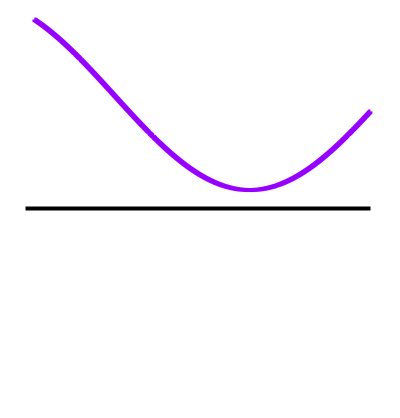
\includegraphics[height=3cm]{trichotomy-1}
  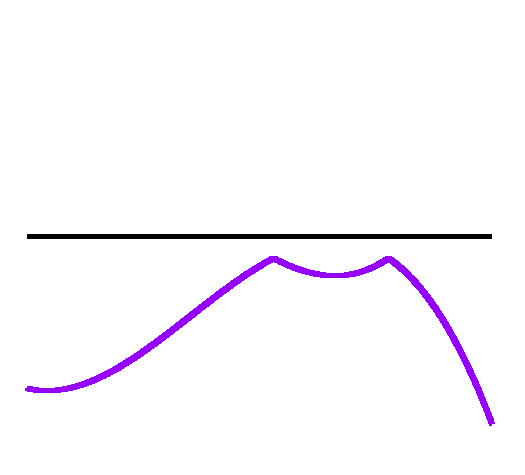
\includegraphics[height=3cm]{trichotomy-2}
  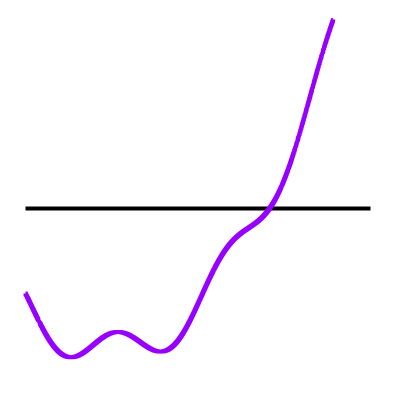
\includegraphics[height=3cm]{trichotomy-3}
  \caption{\label{fig:trichotomy} Three examples of what the topos~$\Sh(X)$
  each believes to be a single real number, where the base space~$X$ is the
  unit interval. (a) A positive real number. (b) A negative real number. (c) A
  number which is neither negative nor zero nor positive. Externally speaking,
  there is no covering of the unit interval by open subsets on which the
  depicted function~$a$ is either everywhere negative, everywhere zero or everywhere
  positive.}
\end{figure}

\begin{figure}
  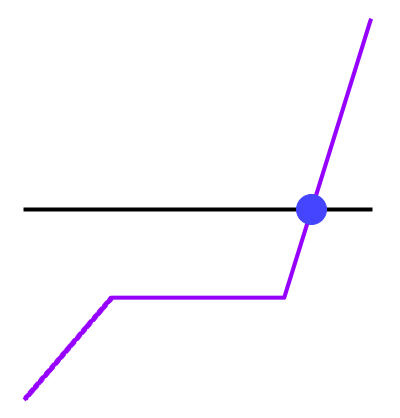
\includegraphics[height=3cm]{zeros-in-families-still}
  \caption{\label{fig:ivt} A single member~$f_{x_0}$ of a continuous
  family~$(f_x)_{x \in X}$ of continuous functions~$f_x : \RR \to \RR$. The
  parameter space is~$X = [0,1]$ (not shown) and the other functions~$f_x$ are
  obtained from~$f_{x_0}$ by moving the horizontal plateau further up or further
  down. The depicted member~$f_{x_0}$ has a unique
  zero and there is an open neighborhood~$U$ of~$x_0$ on which zeros of the
  functions~$f_x$, $x \in U$ can be picked continuously. However, there is no
  such neighborhood of that particular parameter value~$x_1$ for which the
  horizontal plateau lies on the $x$-axis.}
\end{figure}


\subsection{Real functions} Let~$(f_x)_{x \in X}$ be a continuous family of
continuous real-valued functions; that is, each of the individual
functions~$f_x : \RR \to \RR$ should be continuous and moreover the map~$\RR
\times X \to \RR, (a,x) \mapsto f_x(a)$ should be continuous.
From the point of view of~$\Sh(X)$, this family looks like a single continuous
function~$f : \RR \to \RR$.

The internal statement~``$f(-1) < 0$'' means that~$f_x(-1) < 0$ for all~$x \in
X$, and similarly so for being positive. More generally, if~$a$ and~$b$ are
continuous functions~$X \to \RR$ (hence real numbers from the internal point of
view), the internal statement~``$f(a) < b$'' means that~$f_x(a(x)) < b(x)$ for
all~$x \in X$.

The internal statement~``$f$ possesses a zero'', that is ``there exists a
number~$a$ such that~$f(a) = 0$'', means that all the functions~$f_x$ each
possess a zero and that moreover, these zeros can locally be picked in a
continuous fashion. More precisely, this statement means that there is an open
covering~$X = \bigcup_i U_i$ such that, for each index~$i$, there is a continuous
function~$a : U_i \to \RR$ such that~$f_x(a(x)) = 0$ for all~$x \in U_i$. (On
overlaps~$U_i \cap U_j$, the zero-picking functions~$a$ need not agree.)

From these observations we can deduce that the intermediate value theorem of
undergraduate calculus does in general not hold in~$\Sh(X)$ and hence does not allow
for an intuitionistic proof. The intermediate value theorem states: ``If~$f : \RR \to \RR$
is a continuous function such that~$f(-1) < 0$ and~$f(1) > 0$, there exists a
number~$a$ such that~$f(a) = 0$.'' The external meaning of this statement is
that in any continuous family~$(f_x)_x$ of continuous functions with~$f_x(-1) <
0$ and~$f_x(1) > 0$ for all~$x \in X$, it is locally possible to pick zeros of
the family in a continuous fashion. Figure~\ref{fig:ivt} shows a counterexample
to this claim.


\section{Topos adapted to synthetic differential geometry}
\label{sect:smooth}

The idea of \emph{infinitesimal numbers} -- numbers which lie between~$-\frac{1}{n}$
and~$\frac{1}{n}$ for any natural number~$n$ -- has a long and rich history. They are
not part of today's standard setup of the reals, but they are still intriguing
as calculational tools and as a device to bring mathematical intuition and
mathematical formalism closer together.

For instance, employing numbers~$\varepsilon$ such that~$\varepsilon^2 = 0$, we can
compute derivatives blithely as follows, without requiring the notion of
limits:
\begin{equation}\label{eq:derivative}\tag{$\star$}
  \begin{aligned}
    (x + \varepsilon)^2 - x^2 &= x^2 + 2x\varepsilon + \varepsilon^2 - x^2 = 2x\varepsilon \\
    (x + \varepsilon)^3 - x^3 &= x^3 + 3x^2\varepsilon + 3x\varepsilon^2 + \varepsilon^3 - x^3 = 3x^2\varepsilon
  \end{aligned}
\end{equation}
In each case, the derivative is visible as the coefficient of~$\varepsilon$ in
the result. A further example is from geometry: Having a nontrivial
set~$\Delta$ of infinitesimal numbers available allows us to define a
\emph{tangent vector} to a manifold~$M$ to be a map~$\gamma : \Delta \to M$. This
definition precisely captures the intuition that a tangent vector is an
infinitesimal curve.


\subsection{Hyperreal numbers} There are several ways for introducing
infinitesimals into rigorous mathematics. One is Robinson's \emph{nonstandard
analysis}, where we enlarge the field~$\RR$ of real numbers to a
field~$^\star\RR$ of \emph{hyperreal numbers} by means of a non-principal
ultrafilter.

The hyperreals contain an isomorphic copy of the ordinary reals as the
so-called \emph{standard elements}, and they also contain infinitesimal numbers
and their inverses, transfinite numbers. Additionally, they support a powerful \emph{transfer
principle}: Any statement which does not refer to standardness is true for the
hyperreals if and only if it is true for the ordinary reals.

In the ``if'' direction, the transfer principle is useful for importing
knowledge about the ordinary reals in the hyperreal realm. For instance,
addition of hyperreals is commutative because addition of reals is.
By the ``only if'' direction, a theorem established for the hyperreals also
holds for the ordinary reals. In this way, the infinitesimal numbers of
nonstandard analysis can be viewed as a convenient fiction, generating a
conservative extension of the usual setup of mathematics.

However, the realization of this fiction crucically rests on a non-principal
ultrafilter, whose existence requires principles which go beyond the means of
Zermelo--Fraenkel set theory~\textsc{zf}.\footnote{A hyperreal number is
represented by an infinite sequence~$(x_0,x_1,x_2,\ldots)$ of ordinary real
numbers. For instance, the sequence~$(1,1,1,\ldots)$ represents the hyperreal
version of the number~$1$, the sequence~$(1,\frac{1}{2},\frac{1}{3},\ldots)$
represents an infinitesimal number and its inverse~$(1,2,3,\ldots)$ represents
a transfinite number.
%
The sequence~$(1,1,1,\ldots)$ is deemed positive, and so is~$(-1,1,1,1,\ldots)$,
which differs from the former only in finitely many places. But
should~$(1,-1,1,-1,\ldots)$ be deemed positive or negative? Whatever the
answer, our decision has consequences for other sequences. For
instance~$(-1,1,-1,1,\ldots)$ should be assigned the opposite sign
and~$(\tan(1),\tan(-1),\tan(1),\tan(-1),\ldots)$ the same.
%
A non-principal ultrafilter is a set-theoretic gadget which fixes all such
decisions once and for all in a coherent manner. Having such an ultrafilter
available, a sequence~$(x_0,x_1,x_2,\ldots)$ is deemed positive if and only if
the set~$\{i \in \NN \,|\, x_i > 0\}$ is part of the ultrafilter.}
Non-principal ultrafilters cannot be described in explicit terms, and
they are also not at all canonical structures: \textsc{zfc} proves that there
are~$2^{2^{\aleph_0}}$ many~\cite{pospisil:ultrafilters}.

A practical consequence of this nonconstructivity is that it can be hard to
unwind proofs which employ hyperreal numbers to direct proofs, and even where
possible there is no general procedure for doing so.


\subsection{Topos-theoretic alternatives to the hyperreal numbers} Topos theory
provides several constructive alternatives for realizing infinitesimals.
One such is ``cheap nonstandard analysis'' by Terence Tao~\cite{tao:cheap-nsa}.
It is to Robinson's nonstandard analysis what potential infinity is
to actual infinity: Instead of appealing to the axiom of choice to
obtain a completed ultrafilter, cheap nonstandard analysis constructs larger
and larger approximations to an ideal ultrafilter on the go.

The following section presents a (variant of a) topos used in \emph{synthetic differential
geometry}~\cite{kock:sdg,kock:new-methods}. This subject is a further topos-theoretic
approach to infinitesimals which is suited to illustrate the philosophy of toposes
as lenses. A major motivation for the development of synthetic differential
geometry was to devise a rigorous context in which the
writings of Sophus Lie, who freely employed infinitesimals in his seminal
works, can be effortlessly interpreted, staying close to the
original and requiring no coding.


\subsection{The Zariski topos} The starting point is the observation that
while the field~$\RR$ of ordinary real numbers does not contain infinitesimals
(except for zero), the ring~$\RR[\varepsilon]/(\varepsilon^2)$ of \emph{dual
numbers} does. This ring has the cartesian product~$\RR \times \RR$ as its
underlying set and the ring operations are defined such
that~$\varepsilon^2 = 0$, where~$\varepsilon \defeq \langle 0,1 \rangle$:
\[
  \langle a,b \rangle + \langle a',b' \rangle \defeq
  \langle a+a', b+b' \rangle \qquad
  \langle a,b \rangle \cdot \langle a',b' \rangle \defeq
  \langle aa', ab'+a'b \rangle
\]
We write~$\langle a,b \rangle$ more clearly
as~$a+b\varepsilon$.

The dual numbers contain infinitesimal numbers, more precisely \emph{nilsquare
numbers}, namely all numbers of the form~$b \varepsilon$ for~$b \in \RR$, and
they are sufficient to rigorously reproduce derivative computations of
polynomials such as~\eqref{eq:derivative}.

However, the dual numbers are severely lacking in other aspects. Firstly, they
do not contain any nilcubic numbers which are not already nilsquare. These are
required in order to extend calculations like~\eqref{eq:derivative} to second
derivatives, as in
\[ (x+\varepsilon)^3 - x^3 = 3x^2\varepsilon + \frac{1}{2!} 6x
\varepsilon^2. \]
Secondly, the dual numbers contain, up to scaling, only a single infinitesimal
number. Further independent infinitesimals are required in order to deal with
functions of several variables, as in
\[ f(x+\varepsilon,y+\varepsilon') - f(x,y) = D_xf(x,y)\varepsilon +
D_yf(x,y)\varepsilon'. \]
Thirdly, and perhaps most importantly, the ring of dual numbers fails to be a
field. The only invertible dual numbers are the numbers of the form~$a +
b\varepsilon$ with~$a$ invertible in the reals; it is not true that any nonzero
dual number is invertible.

The first deficiency could be fixed by passing
from~$\RR[\varepsilon]/(\varepsilon^2)$ to~$\RR[\varepsilon]/(\varepsilon^3)$
(a ring whose elements are triples and whose ring operations are defined such
that~$\langle0,1,0\rangle^3 = 0$) and the second by passing
from~$\RR[\varepsilon]/(\varepsilon^2)$
to~$\RR[\varepsilon,\varepsilon']/(\varepsilon^2,\varepsilon'^2,\varepsilon\varepsilon')$.
In a sense, both of these proposed replacements are better \emph{stages} than
the basic ring~$\RR[\varepsilon]/(\varepsilon)^2$ or even~$\RR$ itself. However,
similar criticisms can be mounted against any of these better stages, and the
problem that all these substitutes are not fields persists.

\bigskip
\paragraph{Introducing the topos}
The \emph{Zariski topos of~$\RR$},~$\Zar(\RR)$, meets all of these challenges. It
contains a ring~$\RR^\sim$, the so-called \emph{ring of smooth numbers}, which reifies
the real numbers, the dual numbers, the two proposed better stages and indeed
any finitely presented~$\RR$-algebra into a single coherent entity. The
Kripke--Joyal translations rules of~$\Zar(\RR)$ are listed in
Table~\ref{table:zariski}. Any evaluation of an internal statement starts out
with the most basic stage of all, the ordinary reals~$\RR$; then, during the
course of evaluation, the current stage is successively refined to better
stages (further finitely presented~$\RR$-algebras).

For instance, universal quantification~``$\forall x \? \RR^\sim$'' not only refers to
all elements of the current stage, but also to any elements of any refinement
of the current stage. Similarly, negation~``$\neg\varphi$'' does not only mean
that~$\varphi$ would imply~$\bot$ in the current stage, but also that it does
so at any later stage.

For reference purposes only, we include the precise definition of the Zariski topos.
\begin{defn}The \emph{Zariski topos of~$\RR$},~$\Zar(\RR)$, is a certain full subcategory of
the category functors from finitely presented~$\RR$-algebras to sets, namely of
the \emph{Zariski sheaves}. The object~$\RR^\sim$ of~$\Zar(\RR)$ is the tautologous functor~$A \mapsto A$.
\end{defn}

\begin{table}
  \begin{framed}
    \begin{tabbing}
      $\Zar(\RR) \models (\forall f\?\NN^\NN\_ \varphi(n))$ \= \kill
      $\Zar(\RR) \models \varphi$ \> iff $\RR \models \varphi$. \\\\
      $A \models s = t$ \> iff $s = t$ as elements of~$A$. \\
      $A \models \top$ \> iff $1 = 1$ in~$A$. \\
      $A \models \bot$ \> iff $1 = 0$ in~$A$. \\
      $A \models (\varphi \wedge \psi)$ \> iff~$A \models \varphi$ and~$A \models \psi$. \\
      $A \models (\varphi \vee \psi)$ \> iff there exists a partition~$1 = f_1 + \cdots + f_n \in A$ such that, \\
      \> \qquad for each index~$i$, $A[f_i^{-1}] \models \varphi$ or~$A[f_i^{-1}] \models \psi$. \\
      $A \models (\varphi \Rightarrow \psi)$ \> iff for any finitely
      presented~$A$-algebra~$B$, \\
      \> \qquad $B \models \varphi$ implies~$B \models \psi$. \\
      $A \models (\forall x\?\RR^\sim\_ \varphi(x))$ \> iff for any finitely
      presented~$A$-algebra~$B$ and \\
      \> \qquad any element~$x_0 \in B$, $B \models \varphi(x_0)$. \\
      $A \models (\exists x\?\RR^\sim\_ \varphi(x))$ \> iff there exists a partition~$1 = f_1 + \cdots + f_n \in A$ such that, \\
      \> \qquad for each index~$i$, there is an element~$x_0 \in A[f_i^{-1}]$ \\
      \> \qquad such that $A[f_i^{-1}] \models \varphi(x_0)$.
    \end{tabbing}

    \bigskip
    \justify
    A \emph{covering} of an~$\RR$-algebra~$A$ is a family of~$A$-algebras of the
    form~$(A[f_i^{-1}])_i$ such that~$1 = f_1 + \cdots + f_n \in A$.
  \end{framed}
  \bigskip

  \caption{\label{table:zariski} A (fragment of) the Kripke--Joyal translation
  rules of the Zariski topos~$\Zar(\RR)$.}
\end{table}


\paragraph{Properties of the smooth numbers}
As a concrete example, the Kripke--Joyal translation of the statement that~$\RR^\sim$ is a field,
\[ \Zar(\RR) \models \forall x\?\RR^\sim\_ (\neg(x = 0) \Rightarrow \exists y\?\RR^\sim\_ xy = 1), \]
is this:
\begin{indentblock}
For any stage~$A$ and any element~$x \in A$, \\
${\qquad}$ for any later stage~$B$ of~$A$, \\
${\qquad\qquad}$ if for any later stage~$C$ of~$B$ \\
${\qquad\qquad\qquad}$ in which~$x = 0$ holds \\
${\qquad\qquad\qquad}$ also~$1 = 0$ holds, \\
${\qquad\qquad}$ then~$B$ can be covered by later stages~$C_i$ such that, \\
${\qquad\qquad\qquad}$ for each
index~$i$, there is an element~$y \in C_i$ with~$xy = 1$ in~$C_i$.
\end{indentblock}
And indeed, this statement is true. Let a stage~$A$ (a finitely
presented~$\RR$-algebra) and an element~$x \in A$ which fulfills the stated
condition be given. Let~$B$ be any later stage of~$A$ (any finitely
presented~$A$-algebra -- such an algebra is also finitely presented as
an~$\RR$-algebra). Then~$x = 0$ holds in the refinement~$C \defeq B/(x)$.
Hence~$1 = 0$ holds in~$C$. By elementary algebra, this means that~$x$ is
invertible in~$B$. Hence the conclusion holds for the singleton covering
of~$B$ by~$C_1 \defeq B$.

\begin{rem}The Zariski topos can also be set up with an arbitrary commutative
ring~$S$ in place of~$\RR$. The resulting topos~$\Zar(S)$ contains a mirror
image~$S^\sim$ of~$S$, a reification of all finitely presented~$S$-algebras into a
single entity. The computation we just carried out also applies in this
more general context and shows that~$S^\sim$ is a field. It is in this sense that the
topos~$\Zar(S)$ provides a lens through which~$S$ looks like a field.

A small variant of this lens has been used to give a new proof of
\emph{Grothendieck's generic freeness lemma}, a fundamental theorem in
algebraic geometry. The new proof uses the lens to reduce to the case
of fields, where the claim is trivial~\cite[Section~11.5]{blechschmidt:phd}.
\end{rem}

Within~$\Zar(\RR)$, we set~$\Delta \defeq \{ \varepsilon \? \RR^\sim \,|\,
\varepsilon^2 = 0 \}$. Then~$\RR^\sim$ has the following properties:
\begin{enumerate}
\item Law of cancellation: $\forall x \? \RR^\sim\_ \forall y \? \RR^\sim\_ \bigl((\forall
\varepsilon \? \Delta\_ x\varepsilon = y\varepsilon)
\Rightarrow x = y\bigr)$
\item Axiom of micro-affinity: $\forall f \? {\RR^\sim}^\Delta\_ \exists! a \? \RR^\sim\_
\forall \varepsilon \? \Delta\_ f(\varepsilon) = f(0) + a\varepsilon$
\end{enumerate}
The unique number~$a$ in the axiom of micro-affinity deserves to be
called~``$f'(0)$''; this is how we synthetically define the derivative in
synthetic differential geometry.

Having motivated the Zariski topos by the desire to devise a universe with
infinitesimals, the actual ontological status of the infinitesimal numbers in
the Zariski topos is more nuanced. The law of cancellation implies that,
within~$\Zar(\RR)$, it is not the case that zero is the only nilsquare number.
However, this does not mean that there actually \emph{is} a nilsquare number
in~$\RR^\sim$. In fact, any nilsquare number cannot be nonzero, as nonzero numbers are
invertible while nilsquare numbers are not. Hence any nilsquare number in~$\RR^\sim$
is \emph{not not} zero. This state of affairs is only possible in an
intuitionistic context.

\begin{rem}The ring~$\RR^\sim$ of smooth numbers does not coincide with the Cauchy reals,
the Dedekind reals or indeed any well-known construction of the reals
within~$\Zar(\RR)$. This observation explains why~$\RR^\sim$ can satisfy the law of
cancellation even though it is an intuitionistic theorem that the only
nilquadratic number in any flavor of the reals is zero.
\end{rem}


\subsection{Well-adapted models} The Zariski topos of~$\RR$ allows to compute with
infinitesimals in a satisfying manner. However it is not suited as a home for
synthetic differential geometry, a first indication being that in~$\Zar(\RR)$,
any function~$\RR^\sim \to \RR^\sim$ is a polynomial function. Hence important functions such as the
exponential function do not exist in~$\Zar(\RR)$. More comprehensively, the
Zariski topos is not a well-adapted model in the sense of the following
definition.

\begin{defn}\label{defn:well-adapted}A \emph{well-adapted model} of synthetic
differential geometry is a topos~$\E$ together with a ring~$\RR^\sim$ in~$\E$ such
that:
\begin{enumerate}
\item The ring~$\RR^\sim$ is a field.
\item The ring~$\RR^\sim$ validates the axiom of micro-affinity and several related
axioms.
\item There is a fully faithful functor~$i : \mathrm{Mnf} \to \E$ embedding the
category of smooth manifolds into~$\E$.
\item The ring~$\RR^\sim$ coincides with~$i(\RR^1)$, the image of the real line
in~$\E$.
\end{enumerate}
\end{defn}

It is the culmination of a long line of research by several authors that
several well-adapted models of synthetic differential geometry exist~\cite{moerdijk-reyes:models}. By the
conditions imposed in Definition~\ref{defn:well-adapted}, for any such
topos~$\E$ the following transfer principle holds: If~$f,g : \RR \to \RR$ are
smooth functions, then~$f' = g$ (in the ordinary sense of the derivative) if
and only if~$i(f)' = i(g)$ in~$\E$ (in the synthetic sense of the derivative).

Hence the nilquadratic infinitesimal numbers of synthetic differential geometry
may freely be employed as a convenient fiction when computing derivatives.
Because the theorem on the existence of well-adapted models has a constructive
proof, any proof making use of these infinitesimals may mechanically be
unwound to a (longer and more complex) proof which only refers to the ordinary
reals.


\subsection{On the importance of language}

XXX translation unwieldy, lens, view, illustrates custom-tailored, ...

\printbibliography

\end{document}


Outline:


Stuff that should be mentioned:

* XXX Syntactical vs. semantical interpretation
* XXX phone call analogy
* XXX quick overview of the several aspects of toposes (maybe at the end, as an outlook?)
* XXX allowing a switch of perspective
* XXX applications in mathematical practice
* XXX int. logic as common denominator
* XXX arbitrariness of the "standard axioms"
* XXX importance of having an adapted language
* XXX Source https://plato.stanford.edu/entries/category-theory/ for relevant literature
* XXX the internal language as a generalized modal operator
* XXX use the phrase "very rich and very deep" (or similarly) about set theory
* XXX Sven(?)
* XXX Kripke models
* XXX more pointers to topos literature
* XXX Reference for the effective topos
* XXX A topos is more than its semantics
* XXX Reference: Moerdijk
* XXX Check references everywhere (give good pointers)
* XXX toposes are not small (Figure 1)
* XXX internal/external

Send to Georg.
Also Giuseppe Cammarata.

* XXX Mike
* XXX Hamkins multiverse
